%%%%%%%%%%%%%%%%%%%%%%%%%%%%%%%%%%%%%%%%
% Structured General Purpose Assignment
% LaTeX Template
%
% This template has been downloaded from:
% http://www.latextemplates.com
%
% Original author:
% Ted Pavlic (http://www.tedpavlic.com)
%
% Note:
% The \lipsum[#] commands throughout this template generate dummy text
% to fill the template out. These commands should all be removed when 
% writing assignment content.
%
%%%%%%%%%%%%%%%%%%%%%%%%%%%%%%%%%%%%%%%%%

%----------------------------------------------------------------------------------------
%       PACKAGES AND OTHER DOCUMENT CONFIGURATIONS
%----------------------------------------------------------------------------------------

\documentclass{article}

\usepackage{fancyhdr} % Required for custom headers
\usepackage{lastpage} % Required to determine the last page for the footer
\usepackage{extramarks} % Required for headers and footers
\usepackage{graphicx} % Required to insert images
\usepackage{verbatim} % Used for inserting dummy 'Lorem ipsum' text into the template

\usepackage{amsmath}
\usepackage{amssymb}

% Margins
\topmargin=-0.45in
\evensidemargin=0in
\oddsidemargin=0in
\textwidth=6.5in
\textheight=9.0in
\headsep=0.25in 

\linespread{1.1} % Line spacing

% Set up the header and footer
\pagestyle{fancy}
\lhead{\hmwkAuthorName} % Top left header
\chead{\hmwkClass\ : \hmwkTitle} % Top center header
\rhead{\firstxmark} % Top right header
\lfoot{\lastxmark} % Bottom left footer
\cfoot{} % Bottom center footer
\rfoot{Page\ \thepage\ of\ \pageref{LastPage}} % Bottom right footer
\renewcommand\headrulewidth{0.4pt} % Size of the header rule
\renewcommand\footrulewidth{0.4pt} % Size of the footer rule

\setlength\parindent{0pt} % Removes all indentation from paragraphs

%----------------------------------------------------------------------------------------
%       DOCUMENT STRUCTURE COMMANDS
%       Skip this unless you know what you're doing
%----------------------------------------------------------------------------------------

% Header and footer for when a page split occurs within a problem environment
\newcommand{\enterProblemHeader}[1]{
\nobreak\extramarks{#1}{#1 continued on next page\ldots}\nobreak
\nobreak\extramarks{#1 (continued)}{#1 continued on next page\ldots}\nobreak
}

% Header and footer for when a page split occurs between problem environments
\newcommand{\exitProblemHeader}[1]{
\nobreak\extramarks{#1 (continued)}{#1 continued on next page\ldots}\nobreak
\nobreak\extramarks{#1}{}\nobreak
}

\setcounter{secnumdepth}{0} % Removes default section numbers
\newcounter{homeworkProblemCounter} % Creates a counter to keep track of the number of problems

\newcommand{\homeworkProblemName}{}
\newenvironment{homeworkProblem}[1][Problem \arabic{homeworkProblemCounter}]{ % Makes a new environment called homeworkProblem which takes 1 argument (custom name) but the default is "Problem #"
\stepcounter{homeworkProblemCounter} % Increase counter for number of problems
\renewcommand{\homeworkProblemName}{#1} % Assign \homeworkProblemName the name of the problem
\section{\homeworkProblemName} % Make a section in the document with the custom problem count
\enterProblemHeader{\homeworkProblemName} % Header and footer within the environment
}{
\exitProblemHeader{\homeworkProblemName} % Header and footer after the environment
}

\newcommand{\problemAnswer}[1]{ % Defines the problem answer command with the content as the only argument
\noindent\framebox[\columnwidth][c]{\begin{minipage}{0.98\columnwidth}#1\end{minipage}} % Makes the box around the problem answer and puts the content inside
}

\newcommand{\homeworkSectionName}{}
\newenvironment{homeworkSection}[1]{ % New environment for sections within homework problems, takes 1 argument - the name of the section
\renewcommand{\homeworkSectionName}{#1} % Assign \homeworkSectionName to the name of the section from the environment argument
\subsection{\homeworkSectionName} % Make a subsection with the custom name of the subsection
\enterProblemHeader{\homeworkProblemName\ [\homeworkSectionName]} % Header and footer within the environment
}{
\enterProblemHeader{\homeworkProblemName} % Header and footer after the environment
}
   
%----------------------------------------------------------------------------------------
%       NAME AND CLASS SECTION
%----------------------------------------------------------------------------------------

\newcommand{\hmwkTitle}{Homework \ \# 2} % Assignment title
\newcommand{\hmwkDueDate}{Tuesday,\ September\ 26,\ 2017} % Due date
\newcommand{\hmwkClass}{MATH-605} % Course/class
\newcommand{\hmwkClassTime}{} % Class/lecture time
\newcommand{\hmwkAuthorName}{Saket Choudhary} % Your name
\newcommand{\hmwkAuthorID}{2170058637} % Teacher/lecturer
%----------------------------------------------------------------------------------------
%       TITLE PAGE
%----------------------------------------------------------------------------------------

\title{
\vspace{2in}
\textmd{\textbf{\hmwkClass:\ \hmwkTitle}}\\
\normalsize\vspace{0.1in}\small{Due\ on\ \hmwkDueDate}\\
\vspace{0.1in}\large{\textit{\hmwkClassTime}}
\vspace{3in}
}

\author{\textbf{\hmwkAuthorName} \\
        \textbf{\hmwkAuthorID}
        }
\date{} % Insert date here if you want it to appear below your name

%----------------------------------------------------------------------------------------

\begin{document}

\maketitle

%----------------------------------------------------------------------------------------
%       TABLE OF CONTENTS
%----------------------------------------------------------------------------------------

%\setcounter{tocdepth}{1} % Uncomment this line if you don't want subsections listed in the ToC

\newpage
\tableofcontents
\newpage


%----------------------------------------------------------------------------------------
%       PROBLEM 2
%----------------------------------------------------------------------------------------


%\begin{homeworkProblem}[Prob. \Roman{homeworkProblemCounter}] % Roman numerals

%--------------------------------------------


\begin{homeworkProblem}[3.3.1] % Using the problem name elsewhere
\problemAnswer{ % Answer
$X \sim \text{Unif}(\sqrt{n} S^{n-1})$ 

$X$ is rotationally invariant. Consider $\mathbf{x} \in \mathbb{R}^n$ such that $||x_i||_2 = ||x||_2 \forall i \in [1,n]$

\begin{align*}
\mathbb{E}[\sum_{i=1}^n\langle X, x_i\rangle^2] &= n\mathbb{E}[\langle X, x \rangle^2]\\
&= \mathbb{E}[||X||_2^2||x||_2^2]\\
%&= tr(\mathbb{E}[XX^T]) ||x||_2^2\\
%&= tr(I_n) ||x||_2^2\\
&= n ||x||_2^2\\
\implies \mathbb{E}[\langle X, x \rangle^2] &= ||x||_2^2
\end{align*}
and hence $X$ is isotropic
}
\end{homeworkProblem}

\begin{homeworkProblem}[3.3.3] % Using the problem name elsewhere
\problemAnswer{ % Answer
Consider $X_i \sim N(0, \sigma^2)$
\begin{align*}
M_{X_i}(t) &= \mathbb{E}[e^{tX_i}]\\
&= \int_{-\infty}^\infty \frac{1}{\sqrt{2\pi \sigma^2} } e^{tx_i}e^{-\frac{x_i^2}{2\sigma^2}} \\
&= \int_{-\infty}^\infty \frac{1}{\sqrt{2\pi \sigma_i^2} } e^{\frac{t^2\sigma^2}{2}}e^{-(\frac{x_i}{\sigma}-t\sigma)^2} &= e^{\frac{t^2\sigma^2}{2}} \\
\end{align*}

We use uniqueness property of MGF (MGF $\leftrightarrow$ distribution) in the parts that follow.

Part 1.

$ g \sim \mathcal{N}(0, I_n)$
\begin{align*}
\langle g, u \rangle &= u^Tg\\
M_{\langle g, u \rangle}(t) &= e^{\frac{t^2u^Tu}{2}}\\
\implies \langle g, u \rangle &= N(0, u^Tu)\\
&= N(0, ||u||_2^2)
\end{align*}

Part 2.

\begin{align*}
M_{X_i}(t) &= e^{\frac{t^2\sigma_i^2}{2}}\\
M_{\sum X_i}(t) &= e^{\frac{t^2\sum \sigma_i^2}{2}}\\
\implies \sum X_i &= N(0, \sum_i \sigma_i^2)
\end{align*}

Part 3.

$G_{ij} \sim N(0, 1)$. From Part 1 $G_{ij}u_i \sim N(0, u_i^2) = N(0,1)$ $\implies Gu \sim N(0, I_m)$ 


}
\end{homeworkProblem}

\begin{homeworkProblem}[3.3.5] % Using the problem name elsewhere
\problemAnswer{ % Answer


$ X \sim N(0, I_n)$

Part 1.

\begin{align*}
\mathbb{E}[\langle X, u \rangle \langle X, v \rangle] &= \mathbb{E}[u^TX(X^Tv)^T]\\
&= \mathbb{E}[v^TXX^Tu] && [\text{Since  $v^TX$ and $u^TX$ are both scalars}]\\
&= v^T \mathbb{E}[XX^T] u\\
&= v^T u\\
&= \langle u, v \rangle
\end{align*}

Part 2.

\begin{align*}
{||Xu-Xv||^2_{L^2}} &= \mathbb{E}[(u^TX-v^TX)( u^TX-v^TX)^T]\\
&= \mathbb{E}[u^TXX^Tu + v^TXX^Tv - u^TXX^Tv-v^TXX^Tu]\\
&= u^T\mathbb{E}[XX^T]u + v^T\mathbb{E}[XX^T]v - u^T\mathbb{E}[XX^T]v-v^T\mathbb{E}[XX^T]u\\
&= (u-v)(u-v)^T\\
\implies ||Xu-Xv||_{L^2} &= ||u-v||_{L^2}
\end{align*}


}
\end{homeworkProblem}

\begin{homeworkProblem}[3.3.6] % Using the problem name elsewhere
\problemAnswer{ % Answer

From 3.3.5. $\mathbb{E}[\langle G, u \rangle \langle G, v \rangle] = \langle u, v \rangle$ Since $u, v$ are orthogonal $\langle u, v \rangle = 0$
Hence $\mathbb{E}[\langle G, u \rangle \langle G, v \rangle]  = 0$.

Also, $Gu \sim N(0, ||u||_2^)$ and $Gv \sim N(0, ||v||_2^)$ and from above we get 
 $\mathbb{E}[\langle G, u \rangle \langle G, v \rangle]  = 0 = \mathbb{E}[\langle G, u \rangle] = \mathbb{E}[\langle G, v \rangle]$. Since $Gu$ and $Gv$ are both gaussian, and $Gu Gv$ have zero correlation, it implies independence.
}
\end{homeworkProblem}

\begin{homeworkProblem}[3.5.3] % Using the problem name elsewhere
\problemAnswer{ % Answer
I tried a few configurations of $A=A^T$, but couldn't disprove the inequality. E.g. $\frac{1}{3}\begin{pmatrix}
\frac{1}{2} & 1\\
1 & \frac{1}{2}
\end{pmatrix}$ then $\sum|A_{ij}x_ix_j| = \frac{1}{2}(x_1+x_2)^2 + 2x_1x_2 \leq \frac{3}{3} = 1$, however for $u_1 = v_1= \begin{pmatrix}
1\\
0
\end{pmatrix}; u_2=v_2=\begin{pmatrix}
0\\
1
\end{pmatrix}$ $\sum_{A_{ij}u_iu_j} = 1$
}
\end{homeworkProblem}

\begin{homeworkProblem}[3.6.7] % Using the problem name elsewhere
\problemAnswer{ % Answer
Consider a 2 dimensional version of the problem where the $n$ dimensional vector $g$ is projected to the plane which contains $u$ and $v$. Since $g$ is normally distributed, the hyperplane $g$ is now a line and is distributed uniformly over a unit circle. See Figure 1.

For $\langle g, u \rangle$ and $\langle g, v \rangle$ to have opposite signs, the line $g$ passes through between $u$ and $v$ and the probability of this is given by $\frac{\alpha}{\pi}$ where $cos(\alpha) = \langle u, v \rangle$ 

Thus, 
\begin{align*}
\mathbb{E}[sign(g, u) sign(g,v)] &=  -1 \times P(sign(g, u) sign(g,v) = -1) \\
&+ 1 \times P(sign(g, u) sign(g,v) = 1) \\
&= -1(\frac{\arccos{\langle u, v \rangle}}{\pi}) + 1(1-\frac{\arccos{\langle u, v \rangle}}{\pi})\\
&= 1 - 2\frac{\arccos{\langle u, v \rangle}}{\pi}\\
&= 1 - 2(\frac{\pi}{2\pi} - \frac{\arcsin{\langle u, v \rangle}}{\pi} ) & [\because \arcsin \theta + \arccos \theta = \frac{\pi}{2}]\\
&= 2\frac{\arcsin{\langle u, v \rangle}}{\pi}
\end{align*}


}

\end{homeworkProblem}
\begin{figure}
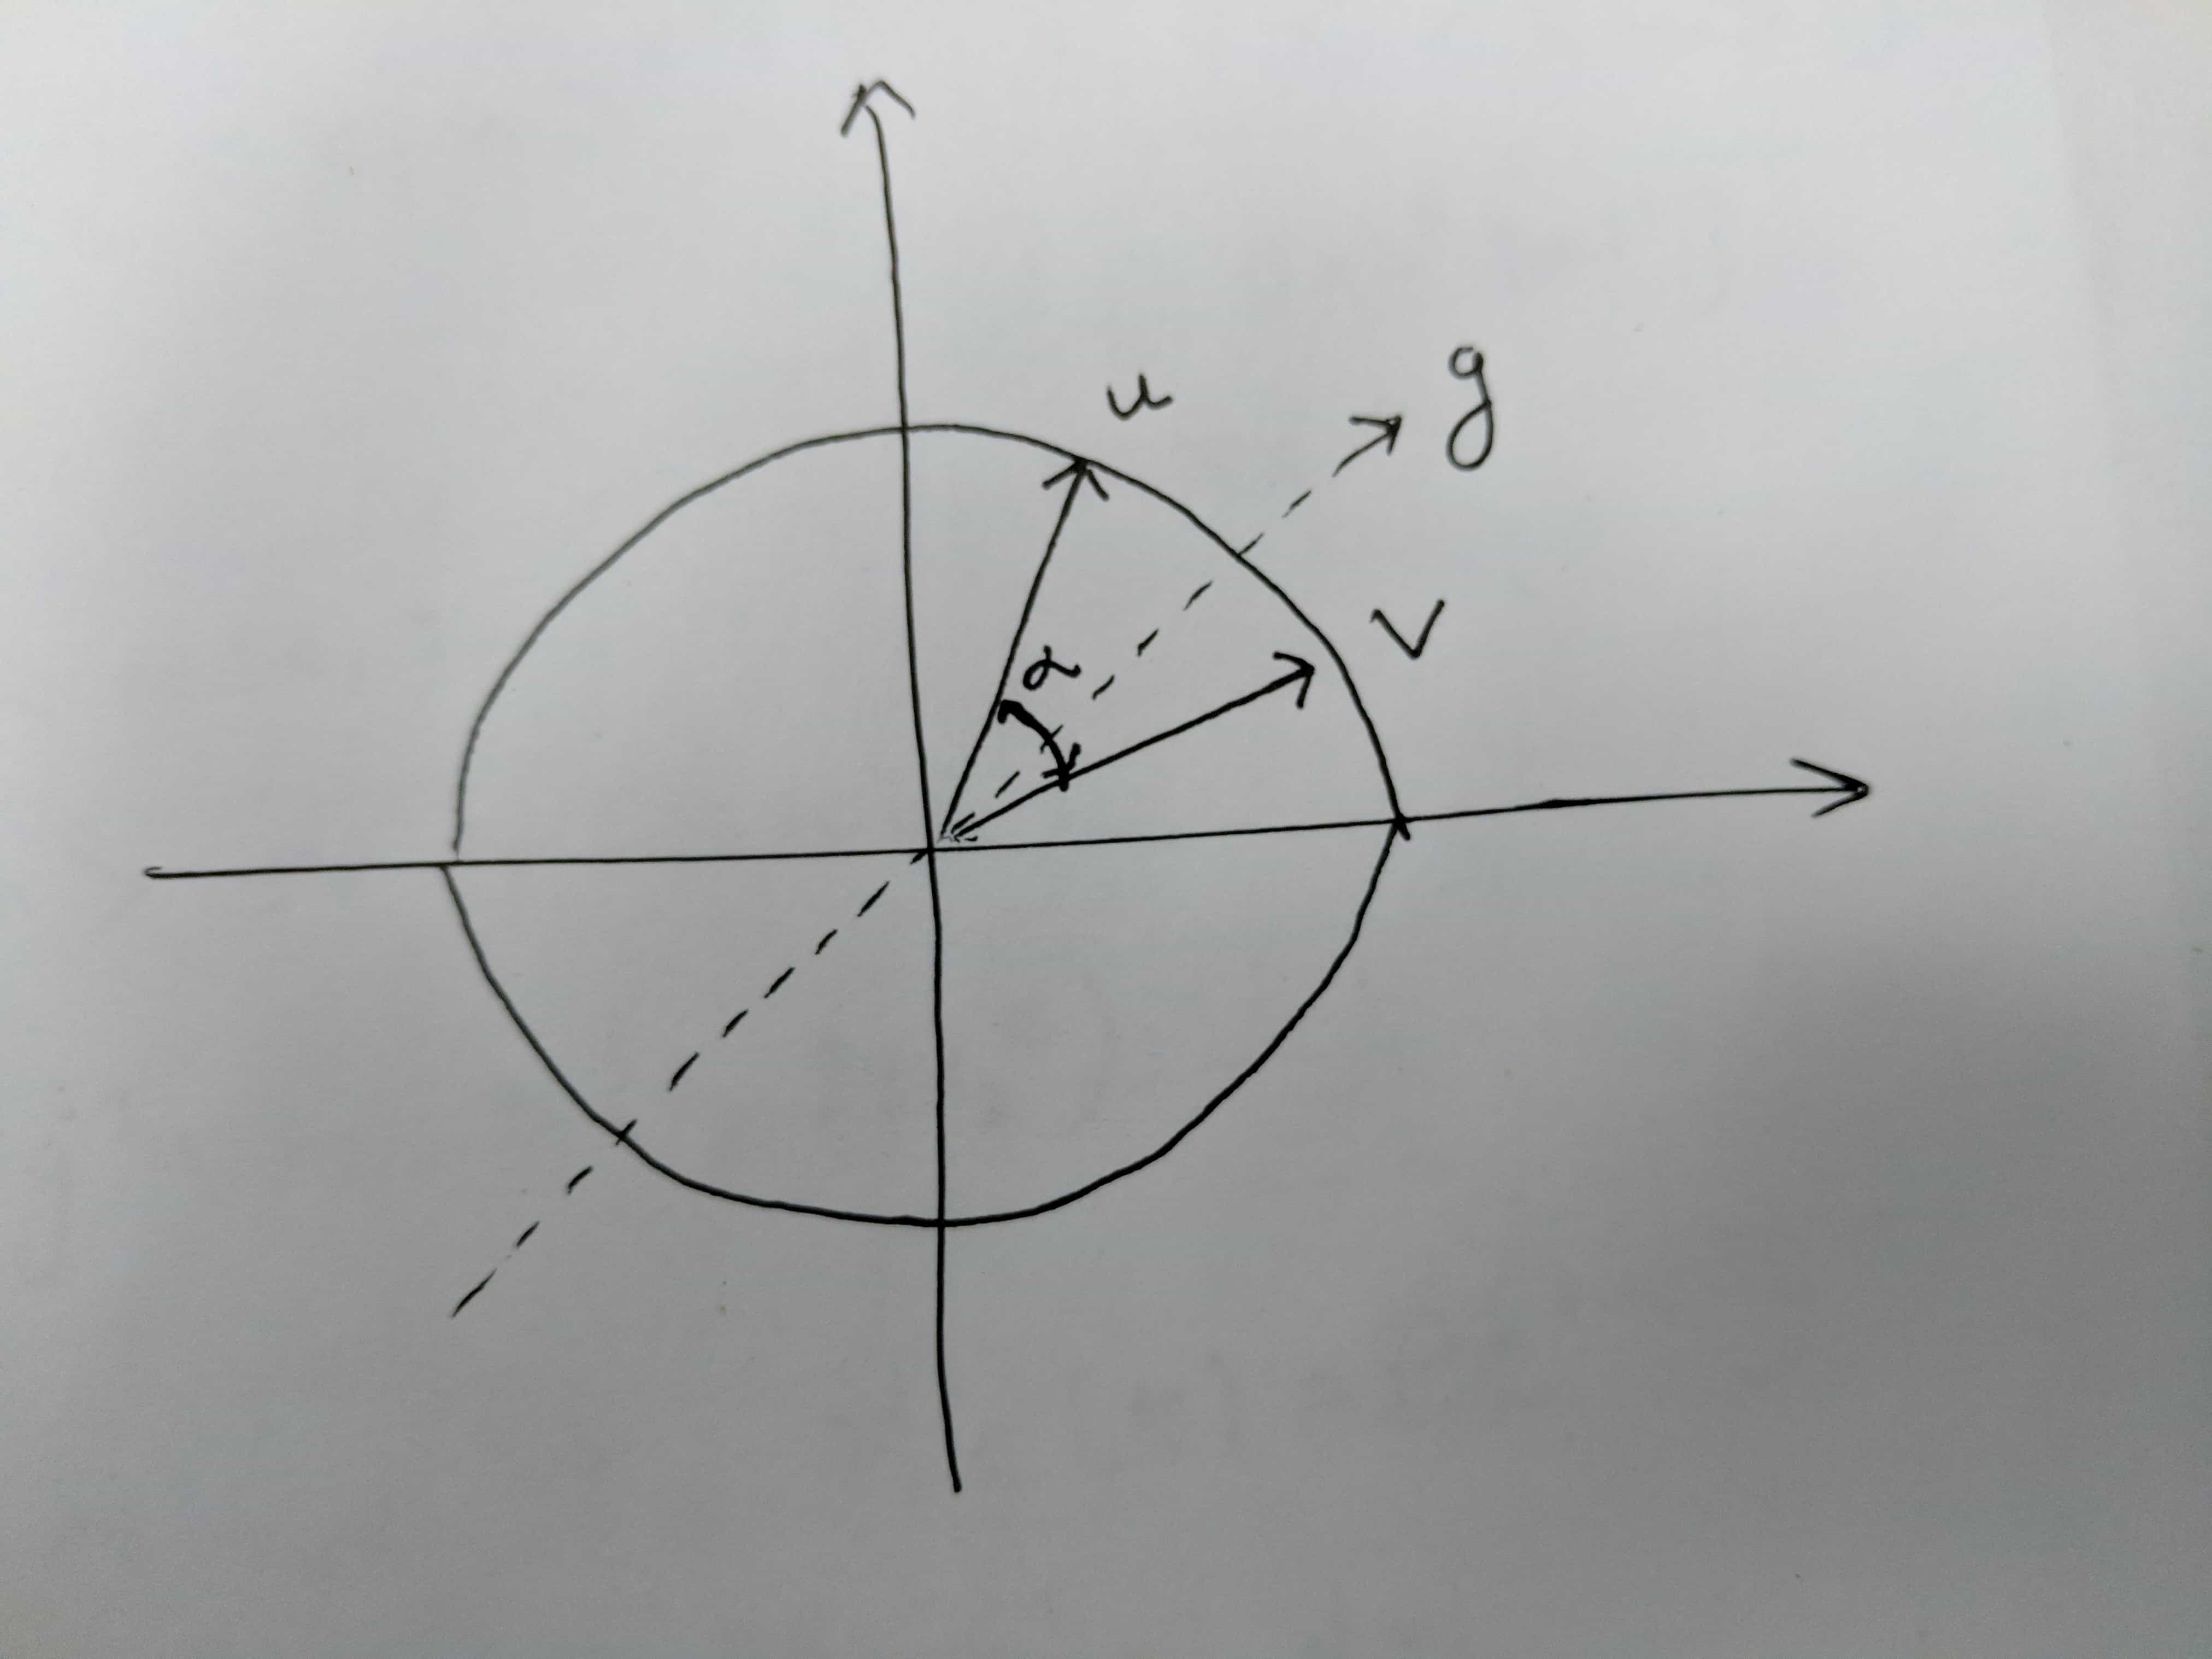
\includegraphics[width=\linewidth]{circle}
\caption{Problem 3.6.7 unit circle. $g$ causes $\langle g, u \rangle$ and $\langle g, v \rangle$ to have opposite sings if it lies in the sector encompassed by $u$ and $v$}
\end{figure}
\begin{homeworkProblem}[3.7.5] % Using the problem name elsewhere
\problemAnswer{ % Answer

Part 1.

Consider $\phi(u)=  \sqrt{2} u \otimes	u \oplus \sqrt{5} u \otimes u \otimes u $ and $\phi(v) = \sqrt{2} v \otimes	v \oplus \sqrt{5} v \otimes v \otimes v$ and $u,v$ are orthogonal.

\begin{align*}
\langle \phi(u), \phi(v) \rangle &= \langle \sqrt{2} u \otimes	u \oplus \sqrt{5} u \otimes u \otimes u, \sqrt{2} v \otimes	v \oplus \sqrt{5} v \otimes v \otimes v \rangle \\
&= \langle \sqrt{2} u \otimes	u, \sqrt{2} v \otimes	v\rangle \oplus  \langle \sqrt{5} u \otimes	u \otimes u, \sqrt{5} v \otimes	v \otimes v \rangle  + 0 \\
&= 2 \langle u \otimes u, v \otimes v \rangle + 5 \langle u \times u \otimes u, v \otimes v \otimes v \rangle \\
&=  2 \langle u , v \rangle^2 + 5 \langle u, v \rangle^3
\end{align*}

Part 2.
\\
For $f(\langle u, v \rangle) = \sum_{i=0}^k a_i \langle u, v \rangle^i$, we let $\phi(u) = \sum_{i=0}^k a_i u^{\otimes i}$ and $\phi(v) = \sum_{i=0}^k v^{\otimes i} $


Part 3.
\\
$f(x) = \sum_{k=0}^{\infty} a_k x^k$, since $a_k > 0$, $\phi(u) = \sum_{k=0}^\infty \sqrt{a_k} u^{\otimes k}$ and $\phi(v) = \sum_{k=0}^\infty \sqrt{a_k} v^{\otimes k}$
}
\end{homeworkProblem}

\begin{homeworkProblem}[3.7.6] % Using the problem name elsewhere
\problemAnswer{ % Answer
Let $\phi(u) = \sum_{k=0}\sqrt{a_k}u^{\otimes k} $ and $\psi(v) = sign(a_k) \sqrt{a_k}v^{\otimes k}$
Then $\langle \phi(u), \psi(v) \rangle = \langle \sum_{k=0}\sqrt{a_k}u^{\otimes k} , \sum_{k=0}sign(a_k)\sqrt{a_k}u^{\otimes k} \rangle = \sum_{k} a_k \langle u , v \rangle^k$ 


Hence $||\phi(u) || = ||\psi(u)|| = \langle  \sum_{k=0}\sqrt{a_k}u^{\otimes k} ,  \sum_{k=0}sign(a_k)\sqrt{a_k}v^{\otimes k} \rangle  = |\sum_{k=0}a_k \langle u, u\rangle ^k |$
}
\end{homeworkProblem}




\end{document}
